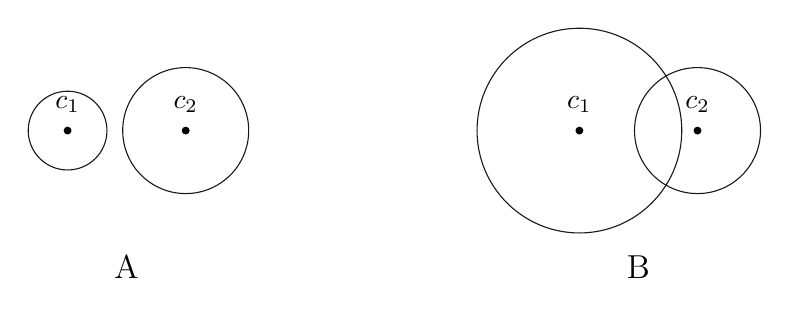
\begin{tikzpicture}[scale=1.0,sty1/.style={color=black!90!white}, sty2/.style={color=blue, line
    width=1.0pt},sty3/.style={color=black, line width=0.6pt}]

%%%%%%%%%%%  Making a helping grid %%%%%%%%%%%%%%%%%%%%%
% \draw[step=0.5cm,gray,very thin] (-5,-5) grid (5,5);
% \foreach \x in {-5,-4,...,5}
% \draw (\x,-5) node[anchor = north,font=\tiny] {\x};
% \foreach \y in {-5,-4,...,5}
% \draw (-5,\y) node[anchor = north,font=\tiny] {\y};
% \draw [sty2] (0,-5) -- (0,5); % y-axis
% \draw [sty2] (-5,0) -- (5,0); % x-axis
%%%%%%%%%%%%%%%%%%%%%%%%%%%%%%%%%%%%%%%%%%%%%%%%%%%%%%%

% Here we have covariance matrices depicted which have off diagonal
% elemenets and thus correspond to a Mahanobis distance. There will be
% ellipses instead of circles:


% Left panel:


%\foreach \r in {0.2,0.4,...,1.3}
\draw[sty1] (-4,0) circle (0.5 cm);
\draw[sty1] (-2.5,0) circle (0.8 cm);
% Center points
\fill[black] (-4,0) circle (0.05 cm);
\fill[black] (-2.5,0) circle (0.05 cm);
% A letter:
\draw (-3.25,-2) node[anchor = south,font=\large] {A};

% Class indicators
\draw (-4,0.1) node[anchor = south,font=\normalsize] {$c_1$};
\draw (-2.5,0.1) node[anchor = south,font=\normalsize] {$c_2$};


% Right panel

\draw[sty1] (2.5,0) circle (1.3 cm);
\draw[sty1] (4,0) circle (0.8 cm);
% Center points
\fill[black] (2.5,0) circle (0.05 cm);
\fill[black] (4,0) circle (0.05 cm);

% Class indicators
\draw (2.5,0.1) node[anchor = south,font=\normalsize] {$c_1$};
\draw (4,0.1) node[anchor = south,font=\normalsize] {$c_2$};


\draw (3.25,-2) node[anchor = south,font=\large] {B};

% Class separation line
%\draw[sty3] (-1-2,0.5) -- (2-2,4.5);

\end{tikzpicture}

